%%%%%%%%%%%%%%%%%%%%%%%%%%%%%%%%%%%%%%
  %%%%%%%%%%%%%%%%%%%%%%%%%%%%%%%%%%%%%%
  % Do not edit the TeX file your work
% will be overwritten.  Edit the RnW
% file instead.
%%%%%%%%%%%%%%%%%%%%%%%%%%%%%%%%%%%%%%
  %%%%%%%%%%%%%%%%%%%%%%%%%%%%%%%%%%%%%%
  
  
      



\begin{knitrout}
\definecolor{shadecolor}{rgb}{0.969, 0.969, 0.969}\color{fgcolor}\begin{figure}[!h]

{\centering 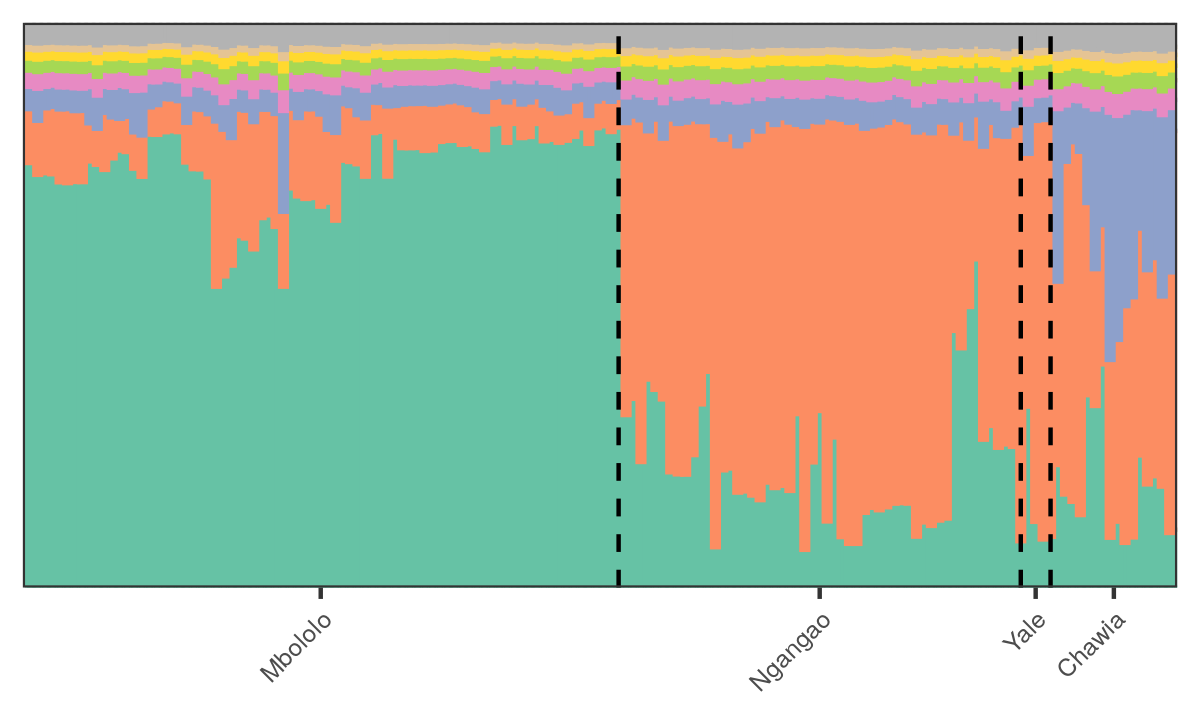
\includegraphics[width=0.98\linewidth,height=0.588\linewidth]{figure/stru_init_fit-1} 

}

\caption[The inferred individual admixtures at alpha = 3]{The inferred individual admixtures at alpha = 3. 
    Each vertical strip is an individual and each color
an ancestral population.
Lengths of colored segments represent the inferred mixture proportions.}\label{fig:stru_init_fit}
\end{figure}


\end{knitrout}

    
    

\begin{knitrout}
\definecolor{shadecolor}{rgb}{0.969, 0.969, 0.969}\color{fgcolor}\begin{figure}[!h]

{\centering 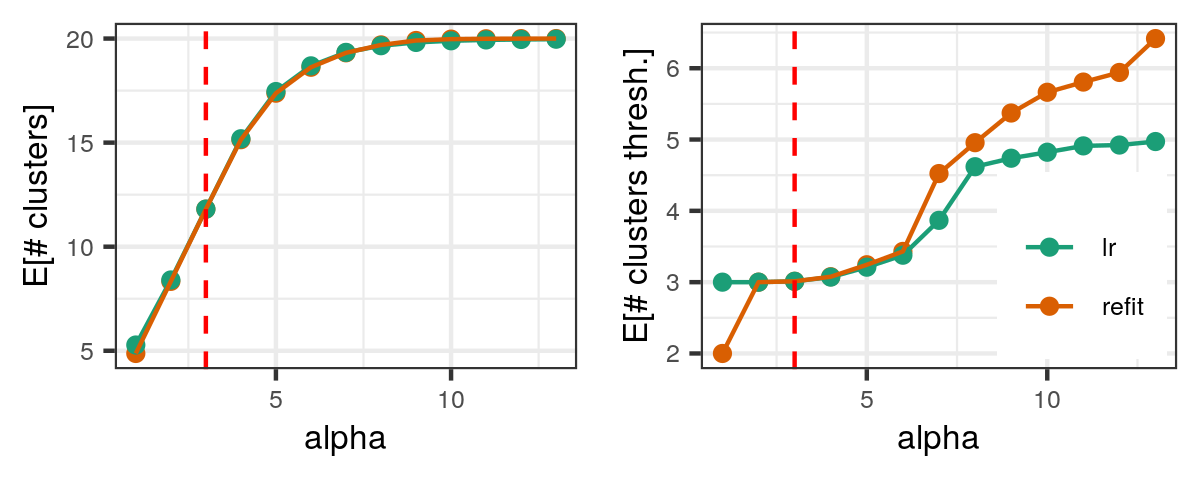
\includegraphics[width=0.98\linewidth,height=0.392\linewidth]{figure/stru_alpha_nclusters-1} 

}

\caption[The expected number of clusters as alpha varies]{The expected number of clusters as alpha varies.  
    We compute the linear approximation at alpha = 3 and
    extrapolate the expected number of clusters from the linear approximation
(green).
We compare against refitting the STRUCTURE model at each alpha (orange).}\label{fig:stru_alpha_nclusters}
\end{figure}


\end{knitrout}




\begin{knitrout}
\definecolor{shadecolor}{rgb}{0.969, 0.969, 0.969}\color{fgcolor}\begin{figure}[!h]

{\centering 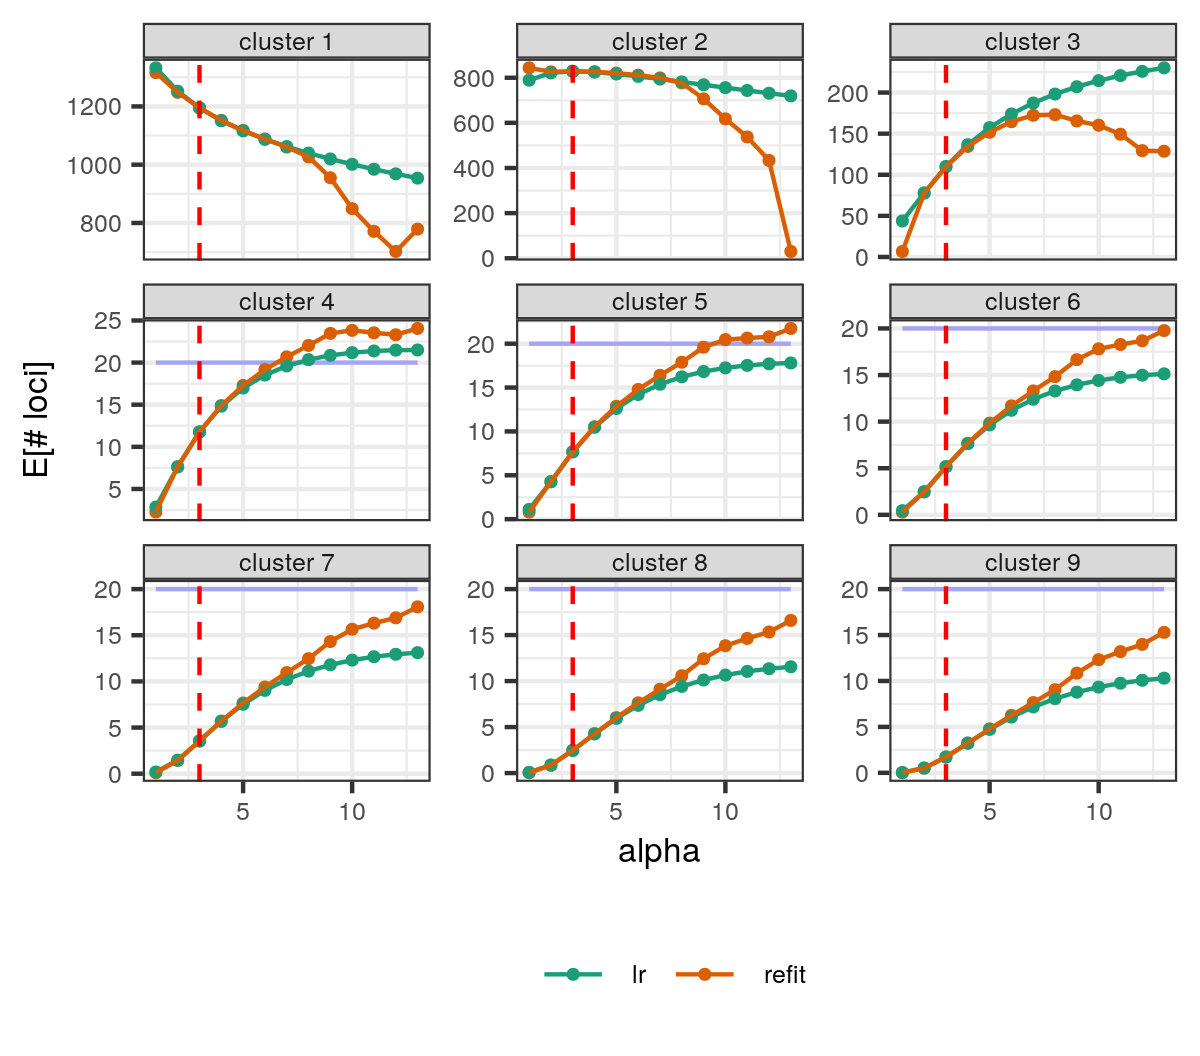
\includegraphics[width=0.98\linewidth,height=0.862\linewidth]{figure/stru_alpha_cluster_weights-1} 

}

\caption[The expected number of loci per cluster as alpha varies]{The expected number of loci per cluster as alpha varies. 
     The horizontal blue line corresponds to the threshold in computing the 
    expected number of clusters in TODO REF. }\label{fig:stru_alpha_cluster_weights}
\end{figure}


\end{knitrout}



\begin{knitrout}
\definecolor{shadecolor}{rgb}{0.969, 0.969, 0.969}\color{fgcolor}\begin{figure}[!h]

{\centering 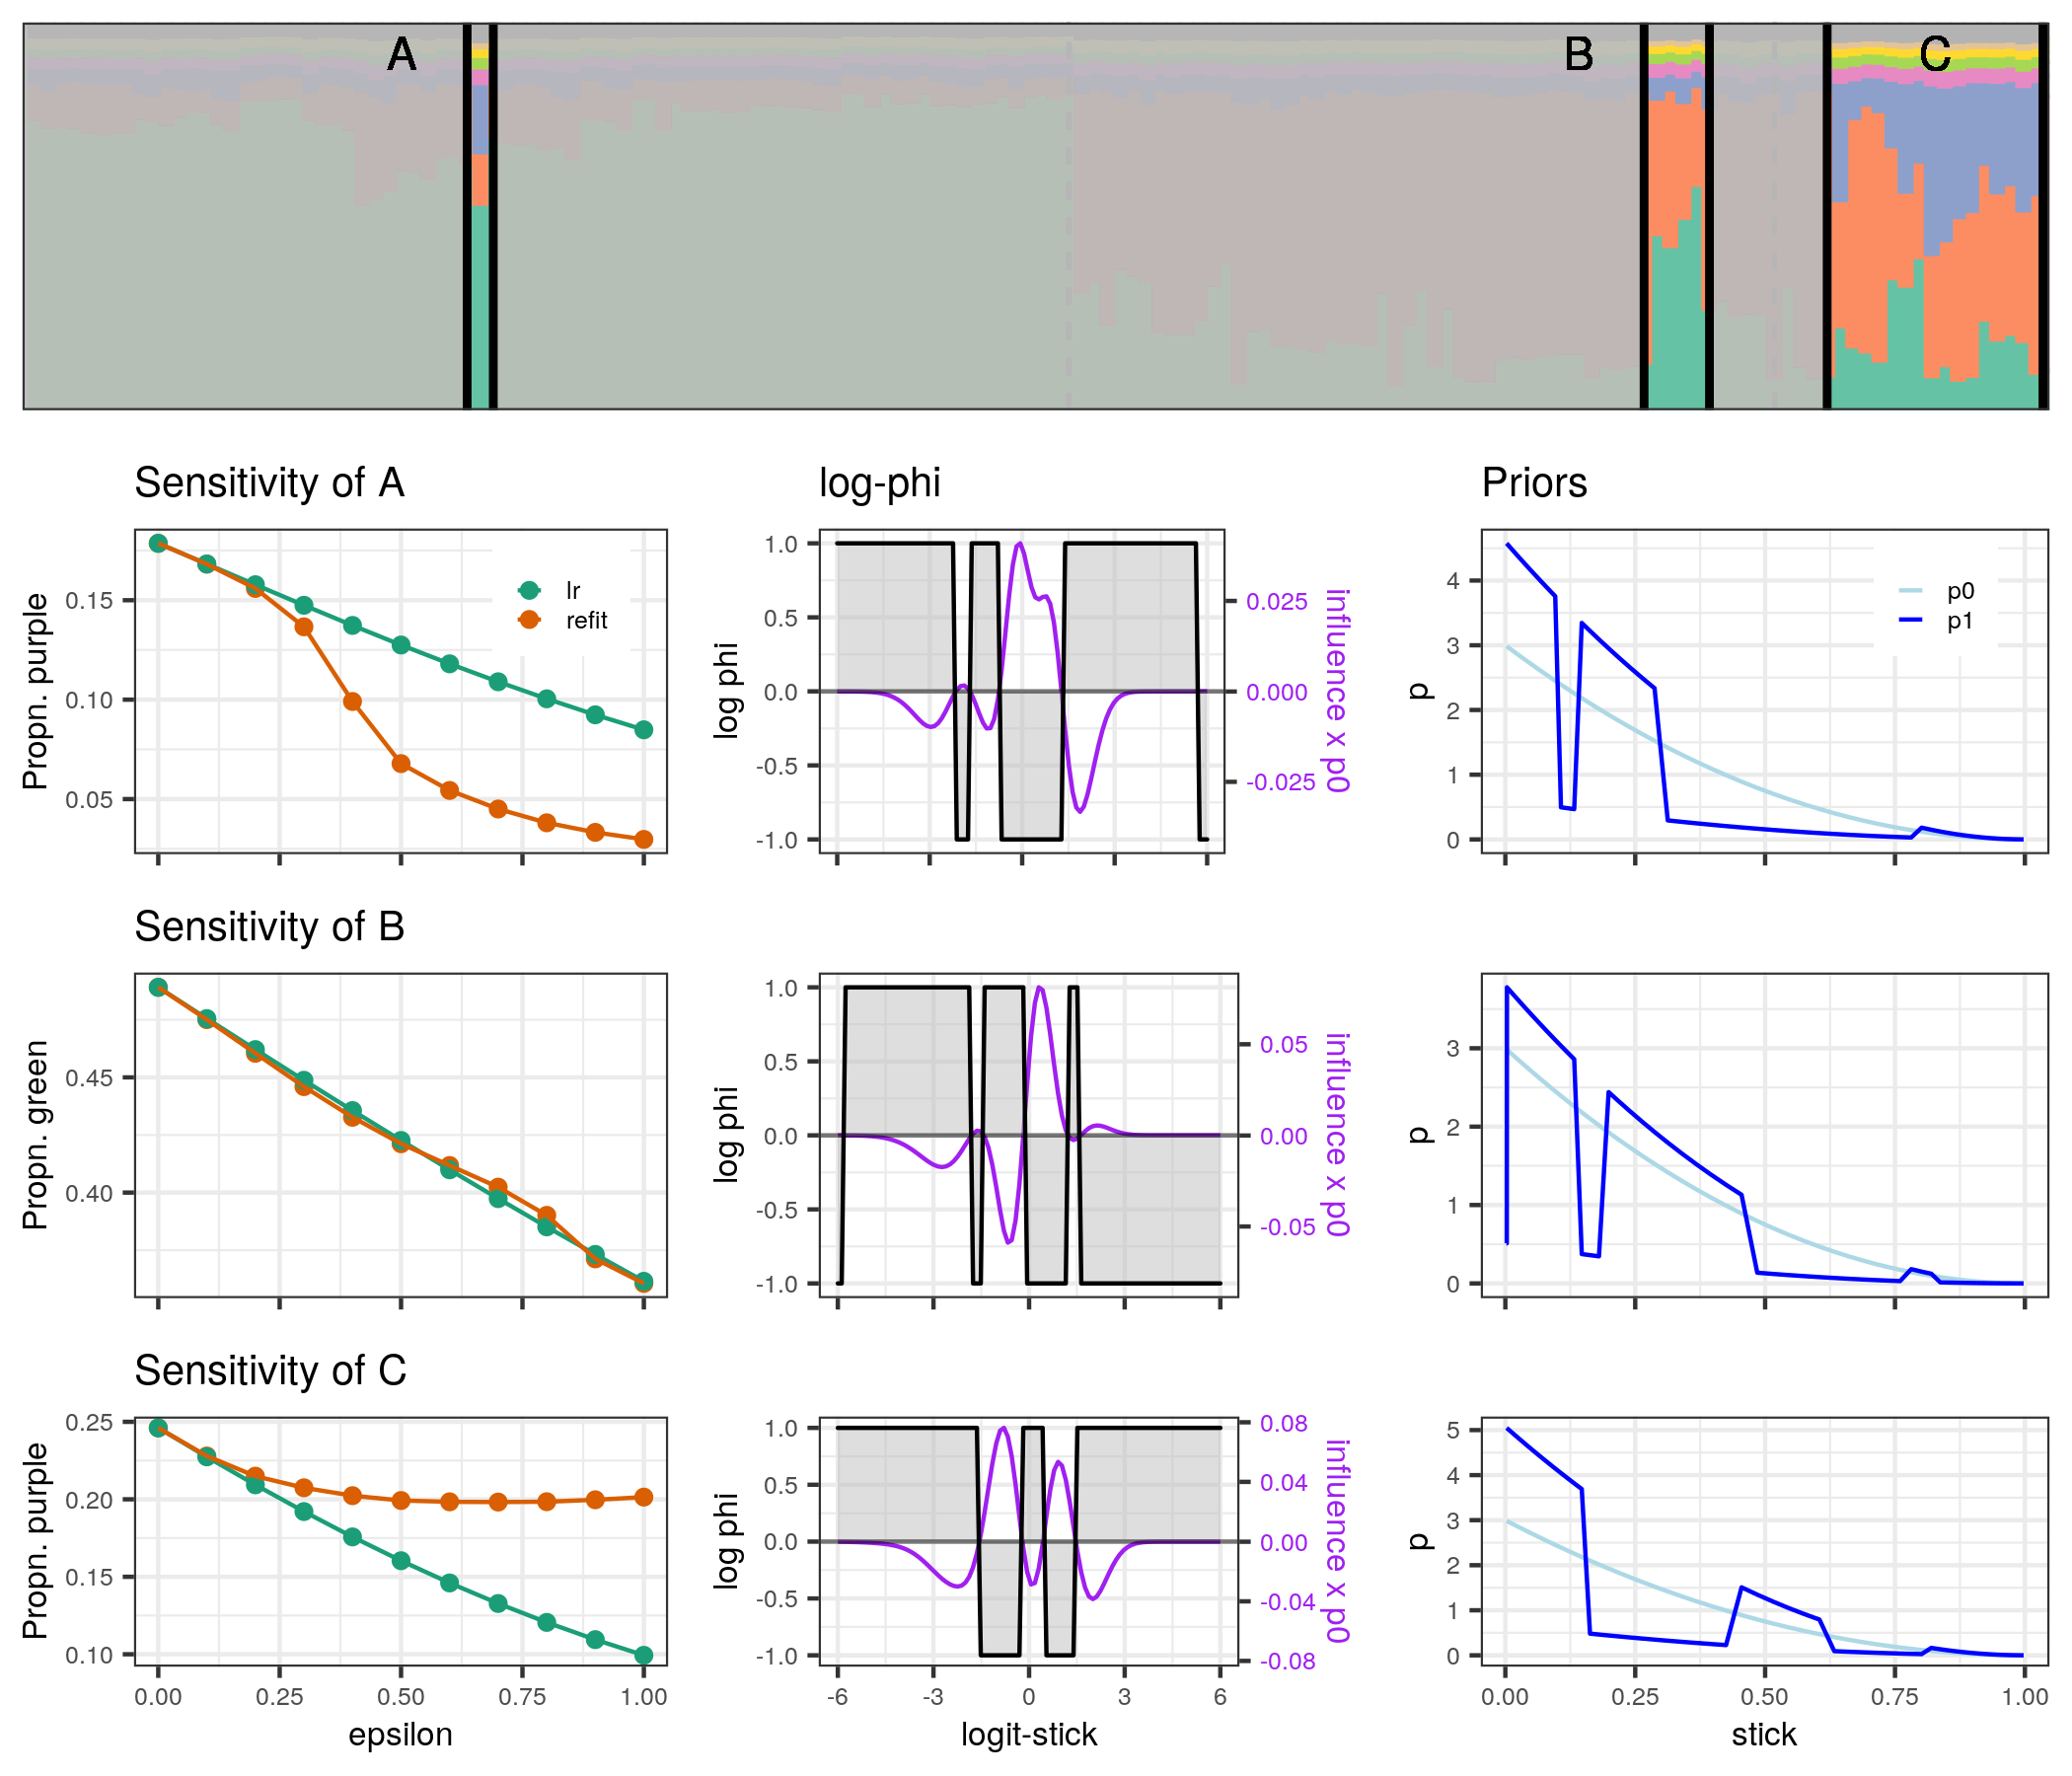
\includegraphics[width=0.98\linewidth,height=0.941\linewidth]{./R_scripts/structure/figures_tmp/fsens_structure} 

}

\caption[structure functional sensitivity ]{structure functional sensitivity }\label{fig:stru_func_sens}
\end{figure}


\end{knitrout}

